\documentclass[aspectratio=169]{beamer}
\usetheme{Madrid}

\usepackage[T1]{fontenc}
\usepackage[utf8]{inputenc}
\usepackage{lmodern}
\usepackage{hyperref}
\usepackage{graphicx}
\usepackage{tikz}
\usetikzlibrary{positioning,arrows.meta}

\graphicspath{{../images/}{../videos/}}
\setbeamertemplate{date}{}
\setbeamertemplate{institute}{}
\beamertemplatenavigationsymbolsempty

\title{Francegen}
\subtitle{Recreating France in Minecraft, block by block:\\a study of GIS, Open Data, and AI-assisted development}
\author{Daniel "defvs" THIRION}
\date{November 28, 2025}

\titlegraphic{%
  \includegraphics[height=0.45\textheight]{puydedome.png}%
}

\begin{document}

\begin{frame}
  \titlepage
\end{frame}

\AtBeginSection[]{
  {%
    \setbeamercolor{background canvas}{bg=blue!70!black}%
    \begin{frame}[plain]
      \centering
      \vfill
      {\color{white}\usebeamerfont{title}\LARGE\insertsection}
      \vfill
    \end{frame}
  }%
}

\begin{frame}{Agenda}
  \tableofcontents
\end{frame}

\section{Motivation}

\begin{frame}{From Idea to Terrain}
  \begin{itemize}
    \item I've always wanted to recreate a massive ski resort in Minecraft.
    \item But Minecraft's default terrain makes mountains small and slopes short.
    \item The in-game scale simply doesn't match real-world topography.
  \end{itemize}
  \begin{center}
    \includegraphics[height=0.5\textheight]{keynote/minecraft_ski.png}

    \vspace{0.1em}
    {\scriptsize My first ski resort, using Terralith generation mod.}
  \end{center}
\end{frame}

\begin{frame}{Problem: Tiny Minecraft Mountains}
  \begin{itemize}
    \item Real ski resorts span tens of kilometers and thousands of meters of elevation.
    \item Vanilla Minecraft height is ridiculously small: 320 blocks tall worlds.
    \item A convincing 1{:}1 experience needs real elevation data or custom generation.
  \end{itemize}
  \begin{center}
    \includegraphics[height=0.6\textheight]{keynote/minecraft_regular_mountains.png}
  \end{center}
\end{frame}

\begin{frame}{Trigger: IGN LIDAR-HD}
  \begin{itemize}
    \item Discovered IGN's LIDAR-HD project: high-resolution LIDAR for all of France.
    \item 50 cm DEMs and dense point clouds available under a free open-data license.
    \item That moment of realization: \emph{“Wait, I can use this for so many things!”}
  \end{itemize}
  \begin{center}
    \includegraphics[height=0.55\textheight]{keynote/lidarhd_example.png}

    % \vspace{0.1em}
    {\scriptsize Viaduc de Millau, France, from LIDAR-HD, \copyright~IGN}
  \end{center}
\end{frame}

\section{Preliminaries}

\begin{frame}{Minecraft in One Slide}
  \begin{itemize}
    \item Sandbox game made of 1\,m blocks, with virtually infinite procedural worlds.
    \item Worlds are stored in chunks and regions; terrain is driven by noise-based generators.
    \item Perfect playground for geodata, if we can control terrain, biomes, and structures.
  \end{itemize}
\end{frame}

\begin{frame}{GIS Basics}
  \begin{columns}[T,onlytextwidth]
    \column{0.6\textwidth}
      \begin{itemize}
        \item Geographic Information Systems (GIS) manage spatial data: rasters, vectors, and point clouds.
        \item Raster DEMs: grids of elevation values (our mountains and valleys).
        \item Vector data: roads, rivers, buildings, and land-use polygons.
        \item Point clouds: dense 3D samples capturing roofs, trees, and terrain details.
        \item Tools and libraries like QGIS make it possible to inspect, slice, and validate these datasets.
      \end{itemize}
    \column{0.4\textwidth}
      \begin{center}
        \includegraphics[width=\linewidth]{keynote/what_is_gis.png}
      \end{center}
  \end{columns}
\end{frame}

\begin{frame}{Overpass API and QL}
  \begin{itemize}
    \item Overpass API is a query language and endpoint for extracting OpenStreetMap data.
    \item Overpass QL lets you filter by tags and geometry: roads, rivers, buildings, POIs, and more.
    \item Queries are small “programs” that describe which ways/nodes/relations to return.
    \item Example: \texttt{way["waterway"="river"];} selects all river ways in the current bounding box.
    \item francegen uses Overpass QL to pull vector data that later gets converted into blocks.
  \end{itemize}
  \begin{center}
    \includegraphics[height=0.45\textheight]{keynote/overpass.png}
  \end{center}
\end{frame}

\section{First Tests}

\begin{frame}{First Prototype: WorldPainter}
  \begin{itemize}
    \item Started with WorldPainter, a GUI tool to design Minecraft worlds.
    \item Imported IGN DEM heightmaps to generate realistic terrain.
    \item Painted biomes manually from satellite imagery to approximate real landscapes.
  \end{itemize}
  \begin{center}
    \includegraphics[height=0.6\textheight]{keynote/worldpainter_screenshot.png}
  \end{center}
\end{frame}

\begin{frame}{Result: Promising but Painful}
  \begin{itemize}
    \item Already looked surprisingly good: recognizable mountains and valleys.
    \item But biomes and details were tedious to paint by hand.
    \item World generation for a single region could take 12+ hours.
    \item Clear conclusion: this needed to be automated and reproducible.
  \end{itemize}
\end{frame}

\section{Implementing francegen}

\begin{frame}{Design Choices}
  \begin{itemize}
    \item Language: \textbf{Rust} --- efficient, safe, and with a rich ecosystem (crates).
    \item Core crates: \texttt{fastnbt}, \texttt{fastanvil}, to work with Minecraft region files; \texttt{tiff} and \texttt{geo} for GIS; \texttt{rayon} for easy multithreading implementation.
    \item CLI-first design to make batch runs and scripting easy.
    \item Not only for France, but France first. Every aspect fully configurable with JSON files.
    \item Coding assistant: OpenAI Codex VSCode extension and GPT-5-Codex series of models.
  \end{itemize}
\end{frame}

\begin{frame}{High-Level Workflow}
  \centering
  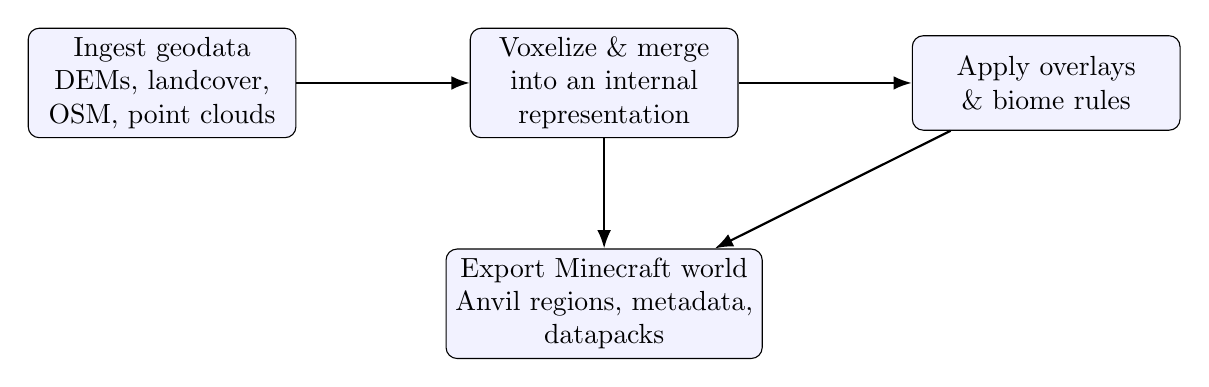
\begin{tikzpicture}[
    node distance=1.4cm and 2.2cm,
    >=Latex,
    box/.style={
      draw,
      rounded corners,
      fill=blue!5,
      align=center,
      minimum width=3.4cm,
      minimum height=1.2cm
    }
  ]
    \node[box] (ingest) {Ingest geodata\\DEMs, landcover,\\OSM, point clouds};
    \node[box, right=of ingest] (voxel) {Voxelize \& merge\\into an internal\\representation};
    \node[box, right=of voxel] (overlay) {Apply overlays\\\& biome rules};
    \node[box, below=of voxel] (export) {Export Minecraft world\\Anvil regions, metadata,\\datapacks};

    \draw[->, thick] (ingest) -- (voxel);
    \draw[->, thick] (voxel) -- (overlay);
    \draw[->, thick] (voxel) -- (export);
    \draw[->, thick] (overlay) -- (export);
  \end{tikzpicture}
\end{frame}

\begin{frame}{Terrain from DEMs}
  \begin{itemize}
    \item Input: GeoTIFF heightmaps in a shared projection (e.g.\ LAMB93).
    \item Resample and normalize elevations to Minecraft's XYZ coordinate range.
    \item Generate base terrain and cliffs at 1{:}1 horizontal and vertical resolution.
  \end{itemize}
  \begin{center}
    \includegraphics[height=0.6\textheight]{keynote/2alpes_heightmap.png}

    % \vspace{0.1em}
    {\scriptsize Les 2 Alpes heightmap, \copyright~IGN}
  \end{center}
\end{frame}

\begin{frame}{OpenStreetMap Data}
  \begin{itemize}
    \item Download OSM data via the Overpass API using Overpass QL queries.
    \item Extract roads, rivers, lakes, boundaries, and building footprints.
    \item Map these features to block palettes and structures in the world.
  \end{itemize}
  \begin{center}
    \includegraphics[height=0.6\textheight]{keynote/2alpes_osm.png}

    \vspace{-0.1em}
    {\scriptsize Les 2 Alpes on OpenStreetMap, \copyright~OpenStreetMap Contributors}
  \end{center}
\end{frame}

\begin{frame}{Landcover and Biomes}
  \begin{columns}[T,onlytextwidth]
    \column{0.5\textwidth}
      \begin{itemize}
        \item Fetch WMTS tiles to obtain landcover and landuse information.
        \item Match tile colors to semantic classes (forest, urban, water, snow, \ldots).
        \item Convert landcover classes into Minecraft biomes and surface blocks.
      \end{itemize}
    \column{0.5\textwidth}
      \begin{center}
        \includegraphics[width=0.6\linewidth]{keynote/cosia_datasheet.png}
      \end{center}
  \end{columns}

  \begin{center}
    \includegraphics[width=0.38\textwidth]{keynote/2alpes_wmts_cosia.png}

    % \vspace{0.1em}
    {\scriptsize Les 2 Alpes landuse, \copyright~IGN}
  \end{center}
\end{frame}

\begin{frame}{Point Clouds to Buildings}
  \begin{itemize}
    \item Ingest COPC point clouds to capture detailed 3D surfaces.
    \item Voxelize points into columns to approximate roofs, facades, and trees.
    \item Use point clouds directly when OSM building heights or shapes are missing.
  \end{itemize}
  \begin{center}
    \includegraphics[width=0.55\textwidth]{keynote/2alpes_lidar.png}

    % \vspace{0.1em}
    {\scriptsize Les 2 Alpes LIDAR-HD, \copyright~IGN}
  \end{center}
\end{frame}

\begin{frame}{Overlays and World Export}
  \begin{itemize}
    \item Apply a stack of overlays (layers) to combine terrain, roads, water, and structures from all sources available.
    \item Write Anvil region files chunk by chunk to disk.
    \item Finalize the world: \texttt{level.dat}, metadata, and a datapack to tweak generation and allow 4096-block-high worlds.
  \end{itemize}
\end{frame}

\begin{frame}[fragile]{Configuration and Customization}
  \begin{itemize}
    \item Everything is customizable through JSON configuration files.
    \item Top and bottom layer blocks, biomes, for each possible layer gathered from the sources.
    \item Example: fetch \verb+way["waterway"]+ from OverpassQL and paint resulting ways with water, width of 2m.
  \end{itemize}
  \begin{center}
    \includegraphics[width=0.5\textwidth]{keynote/json_configuration.png}
  \end{center}
\end{frame}

\begin{frame}{Various challenges and Fixes}
  \begin{itemize}
    \item \textbf{“The world is flat, no trees!”}\\
      Mark chunks as not fully generated so vanilla Minecraft populates trees and features.
    \item \textbf{“Random springs and lava lakes on the surface.”}\\
      Use a datapack to adjust or disable unwanted vanilla features.
    \item \textbf{“OSM buildings are too simple and often lack heights.”}\\
      Fall back to LIDAR point clouds to recover realistic building volumes.
  \end{itemize}
\end{frame}

\begin{frame}{Benchmarks}
  {\scriptsize\textit{Hardware: AMD Ryzen 9 3900X, 64\,GB DDR4, RTX 3070}}%
  % \vspace{0.5em}
  \begin{itemize}
    \item 10\,km $\times$ 10\,km \textbf{Puy de Dôme}:
      \begin{itemize}
        \item $\sim$45 minutes offline generation with francegen.
        \item $\sim$15 minutes additional generation with Chunky in-game.
        {\scriptsize\item $\sim$700MB}
      \end{itemize}
    \item 20\,km $\times$ 8\,km \textbf{Les 2 Alpes}:
      \begin{itemize}
        \item $\sim$2.25 hours offline generation.
        \item $\sim$2 hours online generation
        \item Taller mountains, 600m$\sim$3600m, more blocks to write.
        {\scriptsize\item $\sim$6.7GB}
      \end{itemize}
    \item 4\,km $\times$ 4\,km \textbf{Paris Champs-Elysées}:
      \begin{itemize}
        \item $\sim$7 minutes offline generation
        \item $\sim$4 minutes online generation
        \item Small mountains. Main bottleneck: lots of buildings and LIDAR points
        {\scriptsize\item $\sim$120MB}
      \end{itemize}
    \item Performance is mostly bounded by network, IO and memory.
  \end{itemize}
\end{frame}

\section{In Minecraft}

\begin{frame}{Mods and Environment}
  \begin{itemize}
    \item Mods: Voxy (LODs), C2ME (chunk performance), Chunky (distant world generation).
    \item Hardware: AMD Ryzen 9 3900X, 64\,GB DDR4, RTX 3070.
    \item Goal: be able to locate myself in the world from my own knowledge only.
  \end{itemize}

  \vspace{3em}
  {\scriptsize
    Voxy: \url{https://modrinth.com/mod/voxy}\\
    C2ME: \url{https://modrinth.com/mod/c2me-fabric}\\
    Chunky: \url{https://modrinth.com/plugin/chunky}
  }
\end{frame}

% TODO screenshots

% \begin{frame}{Puy de Dôme}
%   \begin{center}
%     \includegraphics[height=0.4\textheight]{puydedome.png}
%   \end{center}
% \end{frame}

% \begin{frame}{Les 2 Alpes / Venosc}
%   \begin{center}
%     \includegraphics[height=0.4\textheight]{puydedome.png}
%   \end{center}
% \end{frame}

% \begin{frame}{Paris Champs-Elysées}
%   \begin{center}
%     \includegraphics[height=0.4\textheight]{puydedome.png}
%   \end{center}
% \end{frame}

\begin{frame}{Exploring Les 2 Alpes (Live Demo)}
  \begin{itemize}
    \item Live demo
  \end{itemize}
\end{frame}

\section{AI-Driven Development}

\begin{frame}{Toolset and Workflow}
  \begin{itemize}
    \item Coding assistant: OpenAI Codex VSCode extension and GPT-5.1-Codex.
    \item Low budget: \$25 "ChatGPT Plus" monthly subscription.
    \item Workflow: describe intent, generate code, run, debug, iterate.
  \end{itemize}
\end{frame}

\begin{frame}{Why Rust Works Well with LLMs}
  \begin{itemize}
    \item Rust has a large corpus of high-quality open-source code.
    \item Strong type system and compiler errors provide rich feedback loops.
    \item Result: fast iteration cycles with surprisingly robust output.
  \end{itemize}
\end{frame}

\begin{frame}{The Importance of Context}
  \begin{itemize}
    \item You still need to know what you want to build: you become the project head, not the developper.
    \item For obscure formats (like Minecraft's internals), good documentation is crucial.
    \item Example: pasted chunk format details from the Minecraft wiki into the prompt.
    \item The LLM can write code, but it can't run Minecraft, explore worlds, or judge fun.
    \item Progress comes from a tight loop: run, observe, and feed concrete feedback back into the LLM.
  \end{itemize}
\end{frame}

\begin{frame}{Outcome of ``Vibe Coding''}
  \begin{itemize}
    \item All Rust code in this repository was written by LLMs (0 hand-written lines).
    \item Timeline: under 2 weeks of calendar time, roughly 30 hours of focused work.
    \item A lot of that time was spent waiting on the coding agent.
    \item Yet the end result is a complex, working geospatial toolchain with robust code that still, after 2 weeks of work, can be worked on by LLMs without fail.
  \end{itemize}
\end{frame}

\section{Conclusion and Future Work}

\begin{frame}{Successes}
  \begin{itemize}
    \item Biomes, forests, terrain looks amazing.
    \item You can easily recognize the place you are in, even down to the specific ski slope!
    \item These generated worlds are a great starting point for future builds.
  \end{itemize}
\end{frame}

\begin{frame}{Limitations}
  \begin{itemize}
    \item Block resolution is low: hard to capture realistic building facades and fine details.
    \item Lacking texture and material data for true architectural realism.
    \item Point cloud overhangs are challenging; need better algorithms for cliffs and balconies.
    \item Ultimately limited by data sources, data quality, and configuration effort.
  \end{itemize}
\end{frame}

\begin{frame}{Future Directions}
  \begin{itemize}
    \item Use stairs, slabs, and clever block choices to increase apparent resolution.
    \item Experiment with better overhang handling for rocky faces and complex buildings.
    \item Refine presets and configs for more French regions and other countries.
    \item Personally: build a mod for gondolas, ski lifts, and skiing to complete the resort dream.
  \end{itemize}
\end{frame}

\begin{frame}{Thanks}
  \centering Questions? \\
  \vspace{1em}
  Star my repo: \href{https://github.com/defvs/francegen}{github.com/defvs/francegen}
\end{frame}

\end{document}
